\documentclass{article}
\usepackage[utf8]{inputenc}
\usepackage{url}
\usepackage{graphicx}
\usepackage{geometry}
\geometry{a4paper, left=20mm, right=20mm, top=20mm, bottom=20mm}
 \usepackage{float}
 \documentclass[11pt,oneside]{book}
\usepackage[margin=1.2in]{geometry}
\usepackage[toc,page]{appendix}
\usepackage{graphicx}
\usepackage{natbib}
\usepackage{lipsum}
\usepackage{caption}

\begin{document}

\captionsetup[figure]{margin=1.5cm,font=small,labelfont={bf},name={Figure},labelsep=colon,textfont={it}}
\captionsetup[table]{margin=1.5cm,font=small,labelfont={bf},name={Table},labelsep=colon,textfont={it}}
\setlipsumdefault{1}


\begin{titlepage}


% -------------------------------------------------------------------
% You need to edit the details here
% -------------------------------------------------------------------

\begin{center}
{\LARGE College Of Engineering Trivandrum}\\[3cm]
\linespread{1.2}\huge {\bfseries Application Software Development Lab}\\[3cm]
\linespread{1}

\includegraphics[width=5cm]{img/index.jpeg}\\[3cm]
{\Large Abhishek Manoharan\\ S5  CSE Roll No:2\\ TVE17CS002 }\\[1cm]
%{\large \emph{Supervisors:} Vipin Vasu A V ,Thania Kumar , Remya Krishnan}\\ [1cm]% if applicable
%\large A report submitted in partial fulfilment of FOSS Lab final exam \\in Semester 4\\[0.3cm] 
\textit{ }\\[2cm]
Department of Computer Science\\[0.2cm]
\today
\end{center}

\end{titlepage}
\newpage
\tableofcontents
\newpage

\begin{frame}{}
    \centering
    \hspace*{-0.5cm}
    $\vcenter{\hbox{
\includegraphics[width=1.5cm]{img/index.jpeg}}}$
    $\vcenter{\resizebox{0.95\textwidth}{!}{
        \begin{tabular}{c}
             CS333 - Application Software Development Lab $\cdot$ 2019 $\cdot$   \\
             \hline 
        \end{tabular}
    }}$
\end{frame}
\section*{Cycle 1}
\section*{Exp No 1}
\begin{center}
    \Large{INTRODUCTION TO SQL}
\end{center}

\section{Aim}
\large Understand the basics of SQL

\section{Introduction}

SQL is a standard language for accessing and manipulating databases.

\subsection{What is SQL}
\begin{itemize}
   \item SQL stands for Structured Query Language
   \item SQL lets you access and manipulate databases
    \item SQL became a standard of the American National Standards Institute (ANSI) in 1986, and of the International Organization for  Standardization (ISO) in 1987
\end{itemize}
\subsection{What Can SQL do?}
\begin{itemize}
    \item  SQL can execute queries against a database
    \item SQL can retrieve data from a database
    \item SQL can insert records in a database
    \item SQL can update records in a database
    \item SQL can delete records from a database
    \item SQL can create new databases
    \item SQL can create new tables in a database
    \item SQL can create stored procedures in a database
    \item SQL can create views in a database
    \item SQL can set permissions on tables, procedures, and views

\end{itemize}
\subsection{SQL is a Standard - BUT....}

Although SQL is an ANSI/ISO standard, there are different versions of the SQL language.

However, to be compliant with the ANSI standard, they all support at least the major commands (such as SELECT, UPDATE, DELETE, INSERT, WHERE) in a similar manner.

\subsection{RDBMS}
RDBMS stands for Relational Database Management System.

RDBMS is the basis for SQL, and for all modern database systems such as MS SQL Server, IBM DB2, Oracle, MySQL, and Microsoft Access.


\section{History of SQL}

Dr. E. F. Codd published the paper, "A Relational Model of Data for Large Shared Data Banks", in
June 1970 in the Association of Computer Machinery (ACM) journal, Communications of theACM.
Codd's model is now accepted as the definitive model for relational database management systems
(RDBMS). The language, Structured English Query Language ("SEQUEL") was developed by IBM
Corporation, Inc., to use Codd's model. SEQUEL later became SQL (still pronounced "sequel"). In
1979, Relational Software, Inc. (now Oracle Corporation) introduced the first commercially available
implementation of SQL. Today, SQL is accepted as the standard RDBMS language.

\section{How SQL Works}
The strengths of SQL provide benefits for all types of users, including application programmers,
database administrators, managers, and end users. Technically speaking, SQL is a data sublanguage.
The purpose of SQL is to provide an interface to a relational database such as Oracle, and all SQL
statements are instructions to the database. In this SQL differs from general-purpose programming
languages like C and BASIC. Among the features of SQL are the following:
\\
1. It processes sets of data as groups rather than as individual units.\\ \\
2. It provides automatic navigation to the data.\\ \\
3. It uses statements that are complex and powerful individually, and that therefore stand alone.\\ \\
Flow-control statements were not part of SQL originally, but they are found in the recently
accepted optional part of SQL, ISO/IEC 9075-5: 1996. Flow-control statements are commonly
known as "persistent stored modules" (PSM), and Oracle's PL/SQL extension to SQL is
similar to PSM.

SQL unifies all of the above tasks in one consistent language.
Common Language for All Relational Databases
All major relational database management systems support SQL, so you can transfer all skills you
have gained with SQL from one database to another. In addition, all programs written in SQL are
portable. They can often be moved from one database to another with very little modification.
Summary of SQL Statements\\
SQL statements are divided into these categories:\\ \\
1.Data Definition Language (DDL) Statements\\ \\
2.Data Manipulation Language (DML) Statements\\ \\
3.Transaction Control Statements (TCL)\\ \\
4.Session Control Statement\\ \\
5.System Control Statement\\ \\

\section{Managing Tables}
A table is the data structure that holds data in a relational database. A table is composed of rows and
columns.
\par A table can represent a single entity that you want to track within your system. This type of a table
could represent a list of the employees within your organization, or the orders placed for your
company's products.
\par A table can also represent a relationship between two entities. This type of a table could portray the
association between employees and their job skills, or the relationship of products to orders. Within
the tables, foreign keys are used to represent relationships.
\subsection{Creating Tables}
To create a table, use the SQL command CREATETABLE. \\
Syntax:\\
\texttt {\bf CREATE TABLE 'TABLE NAME'('FIELD NAME ' 'DATA TYPE' 'SIZE',..........) }
\subsection{Altering Tables}
1. To add one or more new columns to the table\\
2. To add one or more integrity constraints to a table\\
3. To modify an existing column's definition (datatype, length, default value, and NOTNULL
integrity constraint)\\
4. To modify data block space usage parameters (PCTFREE, PCTUSED)\\
5. To modify transaction entry settings (INITRANS, MAXTRANS)\\
6. To modify storage parameters (NEXT, PCTINCREASE, etc.)\\
7. To enable or disable integrity constraints associated with the table\\
8. To drop integrity constraints associated with the table\\

\section{Data Types}
\subsection{String Data Types}
\begin{figure}[H]
\centering
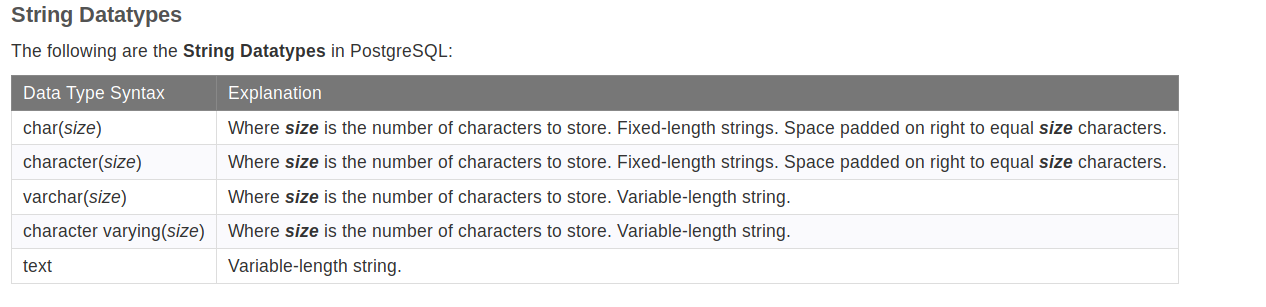
\includegraphics[width=15cm]{1.png}
\caption{String Data Types}\label{delete}
\end{figure}
\section{Result}

\subsection{Numerical Data Types}
\begin{figure}[H]
\centering
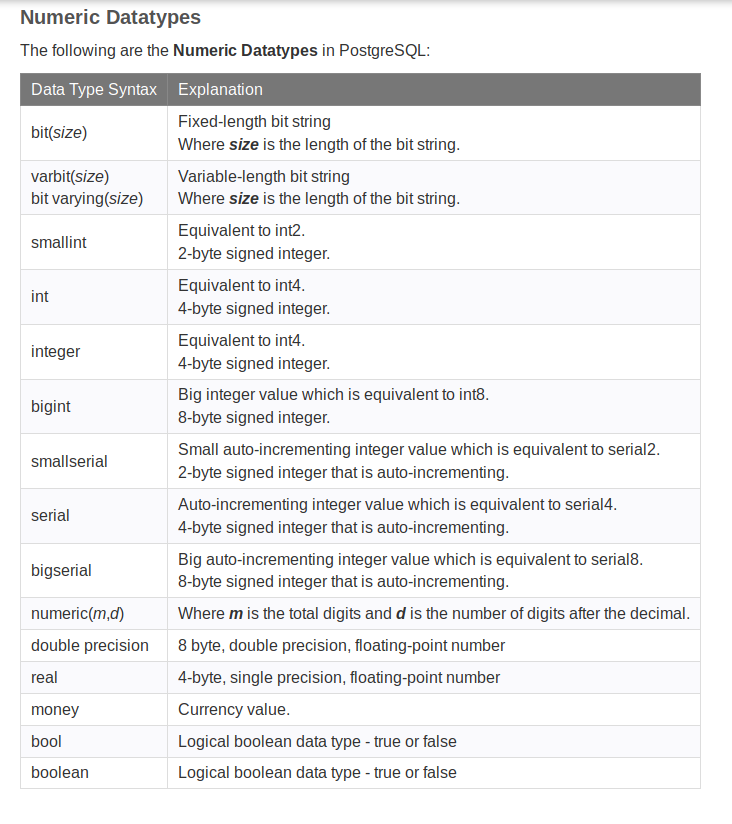
\includegraphics[width=15cm]{2.png}
\caption{Numerical Data Types}\label{delete}
\end{figure}

\subsection{Date/Time Data Types}
\begin{figure}[H]
\centering
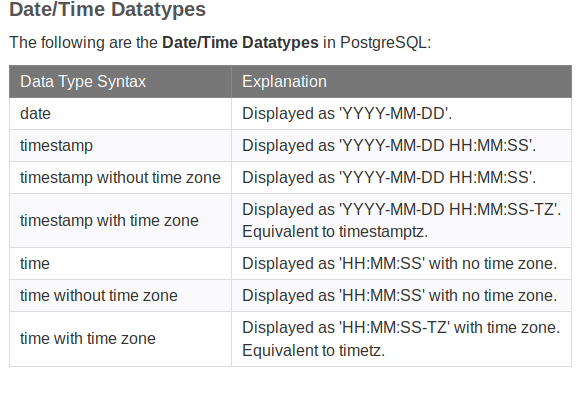
\includegraphics[width=15cm]{3.png}
\caption{Date/Time  Data Types}\label{delete}
\end{figure}


\section{Result}

Understood the basics of SQL.

%\paragraph{Opcional:} Descrição das modificações feitas ao(s) projeto(s) e resultados
%obtidos a partir das mesmas.
 
\end{document}